% Flight / Stay — ATP 2026 DCT Abu Dhabi proposal
% Compile from this directory: tectonic flight_stay_proposal.tex
% Change the team fields below before submission.
% Visual system adapted from the supplied Design Report reference: white
% canvas, black sans-serif headings, generous margins, image-led cover,
% fine rules, restrained warm accent and quiet running footer.
\documentclass[aspectratio=169,10pt]{beamer}
\usepackage[T1]{fontenc}
\usepackage[utf8]{inputenc}
\usepackage[scaled=0.96]{helvet}
\renewcommand{\familydefault}{\sfdefault}
\usepackage{graphicx}
\usepackage{tikz}
\usetikzlibrary{arrows.meta,positioning}
\usepackage{booktabs}
\usepackage{array}
\usepackage{ragged2e}
\usepackage{hyperref}

\definecolor{Ink}{HTML}{171717}
\definecolor{Muted}{HTML}{575757}
\definecolor{Rule}{HTML}{D8D5CF}
\definecolor{Accent}{HTML}{9A7850}
\definecolor{Pale}{HTML}{F5F2ED}
\definecolor{Teal}{HTML}{087E70}
\setbeamercolor{normal text}{fg=Ink,bg=white}
\setbeamercolor{frametitle}{fg=Ink,bg=white}
\setbeamercolor{structure}{fg=Ink}
\setbeamercolor{alerted text}{fg=Accent}
\setbeamertemplate{navigation symbols}{}
\setbeamertemplate{itemize items}[circle]
\setbeamertemplate{frametitle}{%
  \vspace{0.35cm}\insertframetitle\par\vspace{0.07cm}%
  {\color{Rule}\rule{\linewidth}{0.45pt}}\vspace{0.12cm}}
\setbeamertemplate{footline}{%
  \leavevmode\hbox{%
    \begin{beamercolorbox}[wd=.70\paperwidth,ht=.48cm,dp=.12cm,leftskip=.68cm]{normal text}%
      {\color{Muted}\scriptsize FLIGHT / STAY \quad | \quad ATP 2026 · DCT Abu Dhabi}
    \end{beamercolorbox}%
    \begin{beamercolorbox}[wd=.30\paperwidth,ht=.48cm,dp=.12cm,rightskip=.68cm plus1fil]{normal text}%
      {\color{Muted}\scriptsize \hfill \insertframenumber\,/\,10}
    \end{beamercolorbox}}}
\setbeamersize{text margin left=.68cm,text margin right=.68cm}
\setlength{\parskip}{0.18em}

% Fill these in before exporting the final PDF.
\newcommand{\TeamName}{[Team name]}
\newcommand{\MemberOne}{[Name 1]}
\newcommand{\MemberTwo}{[Name 2]}
\newcommand{\MemberThree}{[Name 3]}
\newcommand{\University}{[University / universities]}

\newcommand{\kicker}[1]{{\color{Accent}\scriptsize\bfseries\MakeUppercase{#1}}\par\vspace{.16cm}}
\newcommand{\smallnote}[1]{{\color{Muted}\scriptsize #1}}
\newcommand{\strong}[1]{{\bfseries #1}}
\newcommand{\stat}[2]{%
  {\color{Ink}\fontsize{25}{27}\selectfont\bfseries #1}\par
  {\color{Muted}\small #2}}

\begin{document}

% 1. COVER + EXECUTIVE SUMMARY
\begin{frame}[plain]
  \vspace{.42cm}
  \kicker{Proposal / working prototype}
  {\fontsize{32}{34}\selectfont\bfseries Flight / Stay}\par\vspace{.12cm}
  {\large A flight-to-hotel scenario lab for Abu Dhabi.}\par\vspace{.23cm}
  {\color{Rule}\rule{\linewidth}{.5pt}}\par\vspace{.18cm}
  \begin{columns}[T,totalwidth=\linewidth]
    \begin{column}{.56\linewidth}
      \kicker{Executive summary}
      We built an offline simulator for existing origin markets. Change flights, seats, load factor or connecting share; inspect the demand response.

      On an untouched June--July 2025 audit, nationality-level error fell from \strong{35.0\%} for a calendar-only baseline to \strong{27.7\%}. The slider response still needs causal validation.
    \end{column}
    \begin{column}{.40\linewidth}
      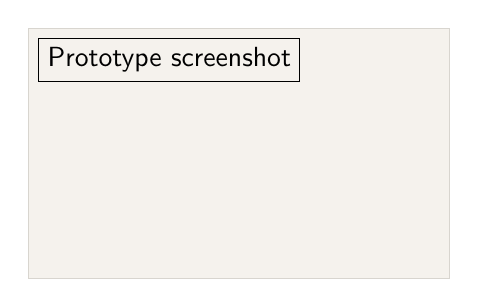
\begin{tikzpicture}
        \begin{scope}
        \clip (0,0) rectangle (5.35,3.18);
        \fill[Pale] (0,0) rectangle (5.35,3.18);
        \node[anchor=north west,inner sep=0] at (.12,3.06)
          {\IfFileExists{assets/demo_baseline.png}{\includegraphics[width=5.10cm]{assets/demo_baseline.png}}{\fbox{Prototype screenshot}}};
        \end{scope}
        \draw[Rule] (0,0) rectangle (5.35,3.18);
      \end{tikzpicture}
      \smallnote{Live prototype. Full view on slide 8.}
    \end{column}
  \end{columns}
  \vfill
  \smallnote{Prepared by \TeamName\quad · \University\quad · October 2026}
\end{frame}

% 2. INTRO / TEAM
\begin{frame}{Who we are and what we built}
  \begin{columns}[T,totalwidth=\linewidth]
    \begin{column}{.50\linewidth}
      \kicker{Student team}
      \begin{tabular}{@{}p{1.75cm}p{4.7cm}@{}}
        \MemberOne & Data preparation and checks \\[.20cm]
        \MemberTwo & Modeling and validation \\[.20cm]
        \MemberThree & Interface and demonstration \\
      \end{tabular}
      \vspace{.55cm}
      \smallnote{Replace these placeholders with the actual team, roles and university before submission.}
    \end{column}
    \begin{column}{.46\linewidth}
      \kicker{Current status}
      \begin{itemize}\setlength\itemsep{.27cm}
        \item Data audit and model comparison notebooks run end to end.
        \item Five interpretable candidates compared on a forward time split.
        \item A working HTML simulator runs locally without a server.
        \item Python predictions and browser slider outputs are checked for agreement.
      \end{itemize}
    \end{column}
  \end{columns}
  \vfill
  {\color{Rule}\rule{\linewidth}{.5pt}}\par
  \smallnote{Our aim is a useful first tool that a planner can question, not an unexplained forecast.}
\end{frame}

% 3. PROBLEM
\begin{frame}{The planning question}
  \kicker{Why this matters}
  \begin{columns}[T,totalwidth=\linewidth]
    \begin{column}{.54\linewidth}
      {\fontsize{21}{24}\selectfont\bfseries If flights change, what happens to hotel demand?}\par\vspace{.20cm}
      Flights and hotels are planned from different datasets. A seat may carry a transfer passenger, a returning resident or a hotel guest. Direct seat-to-room conversion would mislead.
    \end{column}
    \begin{column}{.42\linewidth}
      \kicker{Questions to screen}
      \begin{itemize}\setlength\itemsep{.16cm}
        \item What if weekly frequency rises or falls?
        \item What if an airline uses a larger aircraft?
        \item Which months and markets respond most in the historical data?
      \end{itemize}
    \end{column}
  \end{columns}
  \vfill
  {\color{Accent}\rule{.07cm}{.45cm}}\hspace{.15cm}%
  \smallnote{The challenge asks for a working, transparent, historically tested scenario tool. Source: ATP 2026 DCT Abu Dhabi challenge statement.}
\end{frame}

% 4. DATA AND ASSUMPTIONS
\begin{frame}{The data need an honest bridge}
  \begin{columns}[T,totalwidth=\linewidth]
    \begin{column}{.46\linewidth}
      \kicker{What the files contain}
      \begin{itemize}\setlength\itemsep{.14cm}
        \item Daily flight seats, passengers and connections; daily hotel \emph{Guests} by nationality.
        \item 45 hotel nationalities; 33 have a same-name flight origin.
        \item Hotel \emph{Guests} labels end in July 2025.
      \end{itemize}
    \end{column}
    \begin{column}{.50\linewidth}
      \kicker{Our stated assumptions}
      \begin{itemize}\setlength\itemsep{.14cm}
        \item Same-name origin-to-nationality matching is a provisional link.
        \item The other 12 nationalities use a calendar forecast, with aviation controls disabled.
        \item Monthly \emph{Guests} sums are reported guest-days. Capture, length of stay and occupancy are not separately identified.
      \end{itemize}
    \end{column}
  \end{columns}
  \vspace{.18cm}
  \smallnote{Missing targets are excluded. We start in 2023 because 2022 flight observations have mixed time grain.}
\end{frame}

% 5. SYSTEM DESIGN
\begin{frame}{How the simulator works}
  \kicker{Visible arithmetic, then a fitted response}
  \begin{center}
  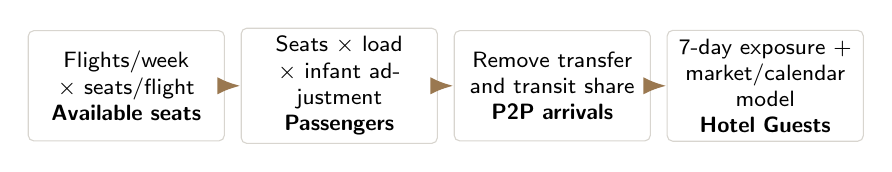
\begin{tikzpicture}[node distance=.20cm,>=Latex,
    box/.style={draw=Rule,fill=white,rounded corners=2pt,align=center,minimum height=1.40cm,text width=2.28cm,inner sep=3pt,font=\footnotesize},
    arr/.style={->,very thick,color=Accent}]
    \node[box] (a) {Flights/week\\$\times$ seats/flight\\\strong{Available seats}};
    \node[box,right=of a] (b) {Seats $\times$ load\\$\times$ infant adjustment\\\strong{Passengers}};
    \node[box,right=of b] (c) {Remove transfer\\and transit share\\\strong{P2P arrivals}};
    \node[box,right=of c] (d) {7-day exposure +\\market/calendar model\\\strong{Hotel Guests}};
    \draw[arr] (a)--(b); \draw[arr] (b)--(c); \draw[arr] (c)--(d);
  \end{tikzpicture}
  \end{center}
  \vspace{.08cm}
  \begin{columns}[T,totalwidth=\linewidth]
    \begin{column}{.48\linewidth}
      \kicker{Inputs}
      Market, month, weekly frequency, seats per flight, load factor and transfer/transit share.
    \end{column}
    \begin{column}{.48\linewidth}
      \kicker{Outputs}
      Predicted reported guest-days, change from observed-flight baseline, daily profile, learned response and extrapolation warning.
    \end{column}
  \end{columns}
  \vfill
  \smallnote{Visitor-to-hotel conversion is absorbed in the fitted response; its individual rate is not identified.}
\end{frame}

% 6. MODEL
\begin{frame}{We chose the simpler model on evidence}
  \begin{columns}[T,totalwidth=\linewidth]
    \begin{column}{.50\linewidth}
      \kicker{Five candidates}
      \begin{enumerate}\setlength\itemsep{.14cm}
        \item Calendar-only baseline
        \item Proportional passenger chain
        \item Monotonic regression \strong{(selected)}
        \item Monotonic GAM, 7-day exposure
        \item Monotonic GAM, stay-kernel exposure
      \end{enumerate}
      \vspace{.2cm}
      \smallnote{The GAMs were slightly worse on the selection period. Extra curve complexity has not earned its place yet.}
    \end{column}
    \begin{column}{.46\linewidth}
      \kicker{Readable response}
      \begin{center}
      \colorbox{Pale}{\parbox{.94\linewidth}{\centering\vspace{.15cm}
        $\log(1+\widehat{G})=\alpha_{m}+\beta_{m}\log(1+P_{7})$\\[.08cm]
        $+\;\text{month}+\text{weekday}+\text{trend}$\\[.08cm]
        $\beta_{m}\geq 0$\vspace{.15cm}}}
      \end{center}
      A separate coefficient for each linked market keeps the passenger response non-decreasing. The seven-day passenger mean lets effects build through the month.
    \end{column}
  \end{columns}
  \vfill
  \smallnote{Selection uses Jan--Apr 2025 only. We favor the simpler eligible model within 1 percentage point of the best WMAPE.}
\end{frame}

% 7. VALIDATION
\begin{frame}{What the back-test actually says}
  \kicker{Lower WMAPE is better}
  \begin{columns}[T,totalwidth=\linewidth]
    \begin{column}{.51\linewidth}
      \small
      \begin{tabular}{@{}p{3.2cm}rr@{}}
        \toprule
        & Calendar & Flight model \\
        \midrule
        Jan--Apr 2025 selection & 31.9\% & \strong{25.0\%} \\[.15cm]
        Jun--Jul 2025 audit & 35.0\% & \strong{27.7\%} \\
        \bottomrule
      \end{tabular}
      \vspace{.20cm}
      \smallnote{WMAPE $=\sum|\text{prediction}-\text{observed}|/\sum\text{observed}$ across nationality-days. Models fit Jan 2023--Dec 2024 after a 27-day warm-up. May 2025 is reserved for error calibration.}
    \end{column}
    \begin{column}{.45\linewidth}
      \kicker{Our reading}
      \stat{7.2 points}{Less error on the untouched audit.}
      \vspace{.18cm}
      \stat{27.7\%}{Too much error for precise market claims.}
    \end{column}
  \end{columns}
  \vfill
  \smallnote{Aggregate daily WMAPE is 6.5\% because market errors can cancel. Validation uses observed flights, not randomized changes.}
\end{frame}

% 8. MOCK-UP / PROTOTYPE
\begin{frame}{A working prototype, not just a diagram}
  \begin{columns}[T,totalwidth=\linewidth]
    \begin{column}{.53\linewidth}
      \kicker{What a planner can do now}
      \begin{enumerate}\setlength\itemsep{.17cm}
        \item Pick an existing origin market and month.
        \item Move a slider for frequency, aircraft seats, load factor or connecting share.
        \item Compare scenario and observed-flight baseline; inspect the passenger chain and demand curve.
        \item See a warning if the scenario leaves the training range.
      \end{enumerate}
      \vspace{.25cm}
      \smallnote{The prototype is a single offline HTML file. Model export and browser calculations are checked against Python.}
    \end{column}
    \begin{column}{.43\linewidth}
      \centering
      \IfFileExists{assets/demo_baseline.png}{%
        \fbox{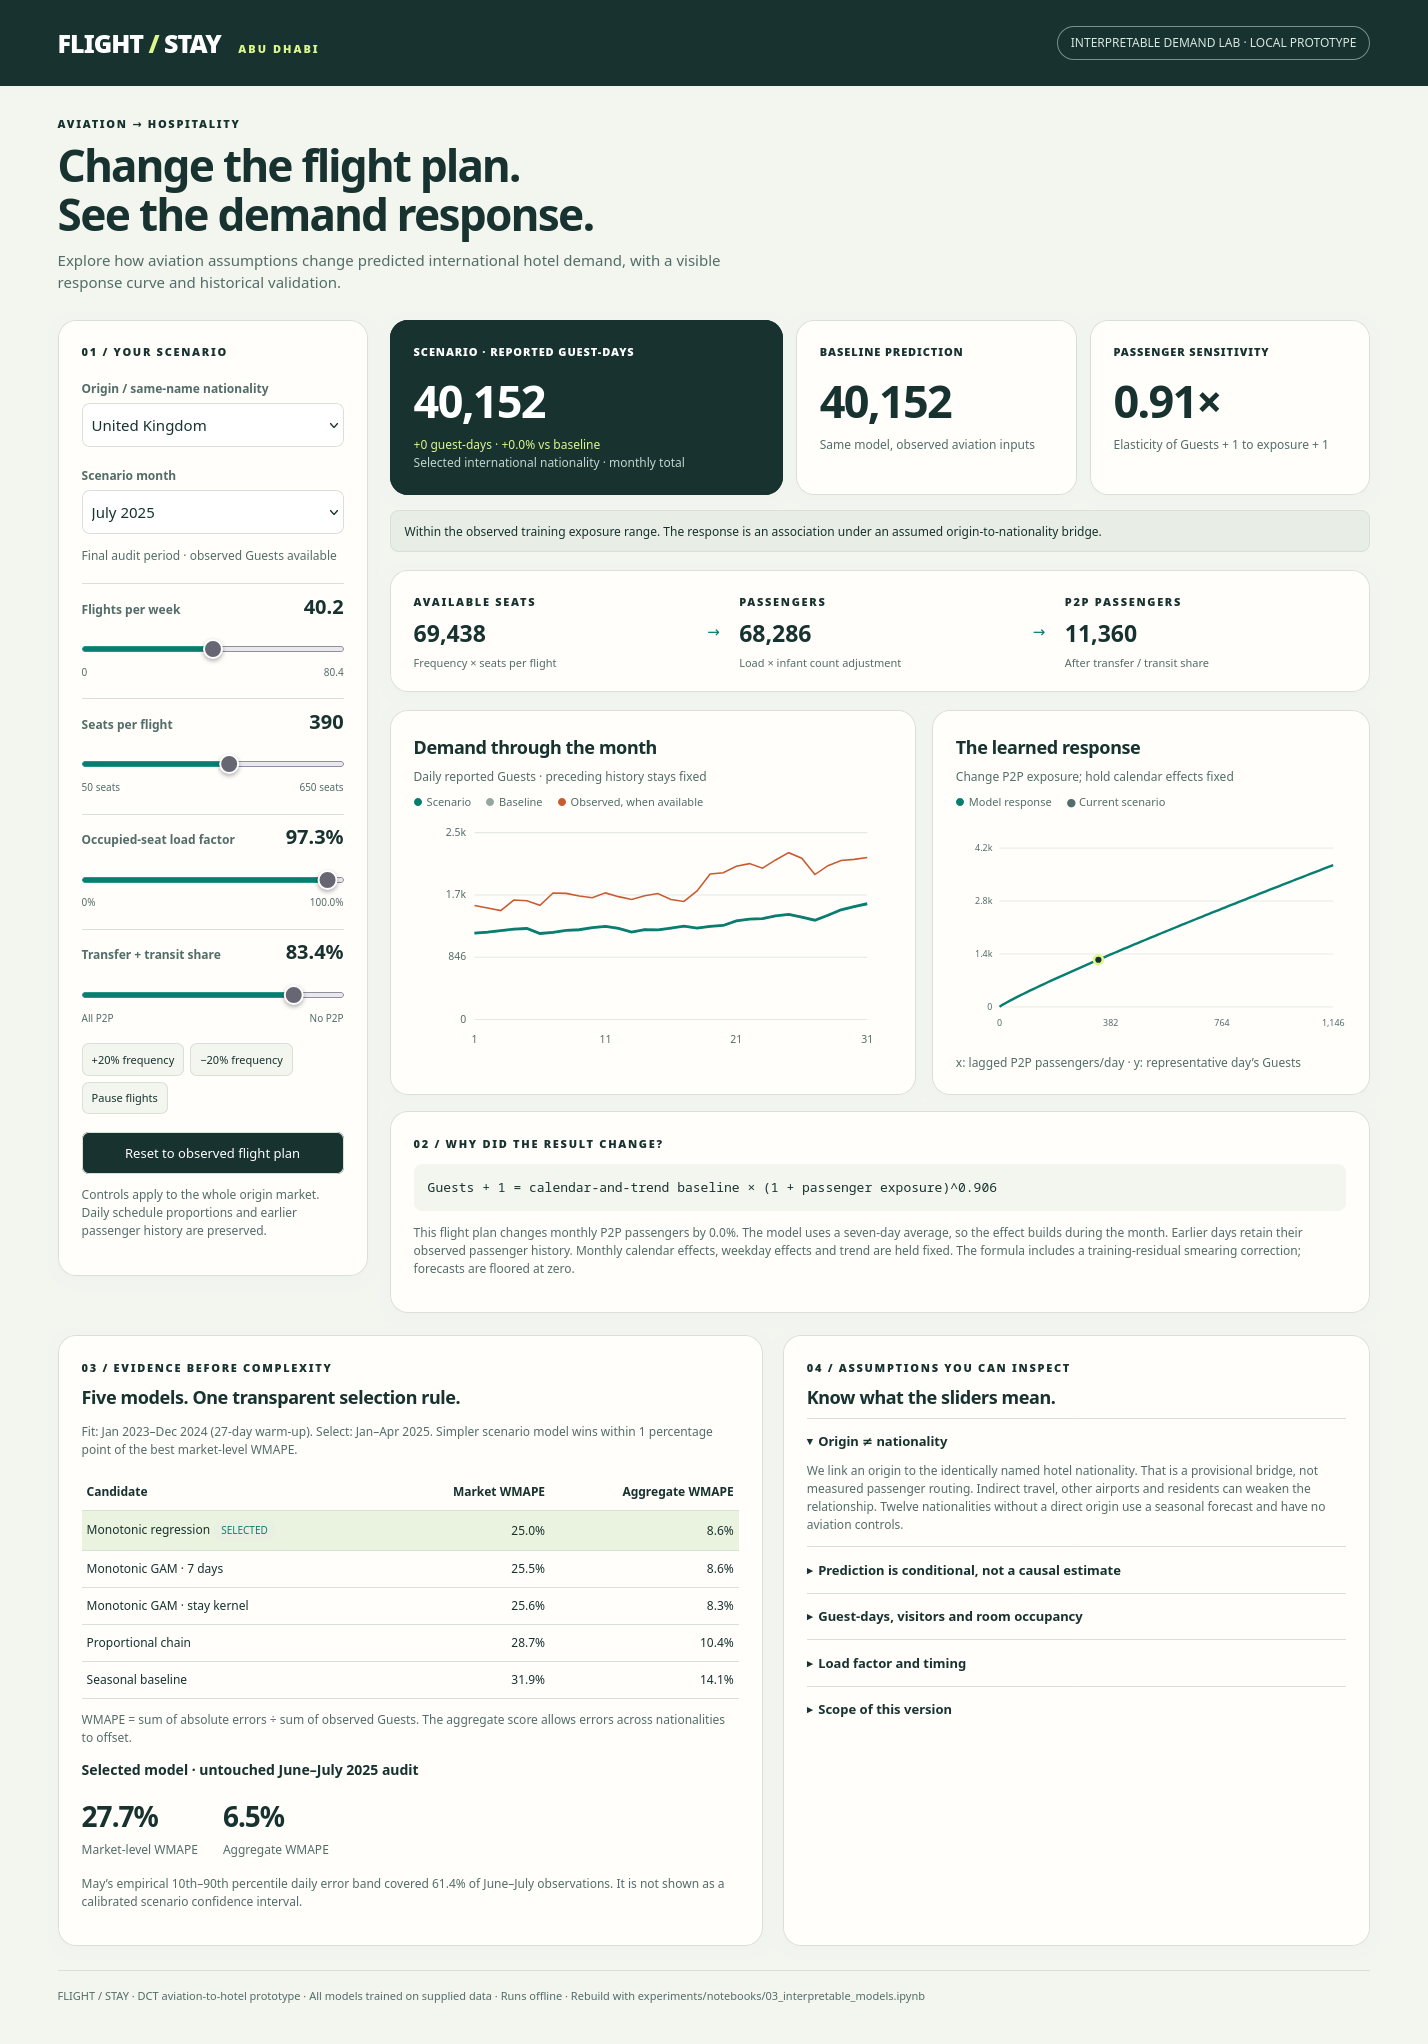
\includegraphics[height=5.65cm]{assets/demo_baseline.png}}%
      }{\fbox{\parbox[c][5.4cm][c]{5cm}{\centering Screenshot: prototype with four sliders and prediction cards}}}
      \par\smallnote{Current HTML prototype, UK / July 2025.}
    \end{column}
  \end{columns}
\end{frame}

% 9. IMPACT AND FEASIBILITY
\begin{frame}{Where this could be useful}
  \begin{columns}[T,totalwidth=\linewidth]
    \begin{column}{.47\linewidth}
      \kicker{Intended impact}
      \begin{itemize}\setlength\itemsep{.16cm}
        \item Make flight and hotel planning assumptions visible in one place.
        \item Compare existing-market scenarios quickly before deeper analysis.
        \item Flag high-sensitivity months and markets for human review.
      \end{itemize}
    \end{column}
    \begin{column}{.49\linewidth}
      \kicker{Real-life requirements}
      \begin{itemize}\setlength\itemsep{.16cm}
        \item Confirm the hotel's \emph{Guests} definition and obtain room inventory for occupancy.
        \item Improve the departure-origin to nationality bridge with approved aggregated data.
        \item Refresh source data and monitor errors by market and season.
        \item Gate unsupported new routes until a defensible prior is available.
      \end{itemize}
    \end{column}
  \end{columns}
  \vfill
  {\color{Rule}\rule{\linewidth}{.5pt}}\par
  \smallnote{The current slider output is an association under stated assumptions; it is not a verified causal effect of adding flights.}
\end{frame}

% 10. SHORTLIST TEST PLAN + SOURCES
\begin{frame}{If shortlisted: test the hard part}
  \begin{columns}[T,totalwidth=\linewidth]
    \begin{column}{.57\linewidth}
      \kicker{Demonstration and validation plan}
      \begin{enumerate}\setlength\itemsep{.12cm}
        \item Demo a baseline, a 20\% frequency increase and a flight cut in the same market/month.
        \item Ask DCT to confirm target definitions and the origin-to-nationality mapping.
        \item Predefine new time periods and actual route-change cases; test model error and the direction of change.
        \item Report failures by market, season and extrapolation level; revise only with a fresh untouched period.
      \end{enumerate}
    \end{column}
    \begin{column}{.39\linewidth}
      \kicker{What we need to improve}
      Aggregated origin--nationality flows, confirmed hotel guest-night definitions, event dates and room inventory. These would let us test more of the requested seats-to-visitors-to-nights chain.

      \vspace{.40cm}
      \smallnote{Prototype and notebooks are ready for a live walkthrough. Team details and final video link should be inserted before submission.}
    \end{column}
  \end{columns}
  \vfill
  {\color{Rule}\rule{\linewidth}{.5pt}}\par
  \tiny Sources: ATP 2026 DCT Abu Dhabi challenge statement (challengeon.atrc.ae); supplied DCT aviation and hotel files; our executed domain analysis and model-comparison notebooks. Results reproduced 11 October 2026.
\end{frame}

\end{document}
